\documentclass{article}
\usepackage [left=22 mm,top=0.5in,bottom=1in]{geometry}
\usepackage[pdftex]{graphics}
\usepackage{amsmath}
\usepackage{amssymb}
\usepackage{caption}
\usepackage{graphicx}
\usepackage{steinmetz}
\usepackage{xpatch}
\usepackage{esint}
\usepackage{gensymb}

\newcommand*\VF[1]{\mathbf{#1}}
\newcommand*\dif{\mathop{}\!\mathrm{d}}

\begin{document}


\begin{center}
		%\line(1,0){400}\\
		%[0.18in]
		\huge{EED4106 ANTENNAS AND PROPAGATION LABORATORY REPORT}\\
		%[0.02mm]
		%\line(3,0){400}\\
	\end{center}

	\begin{center}
		\begin{tabular}{llll}
			\hline
			Name-Surname:Efe Kiraz & Student ID:2016502071 & Date of Laboratory:31/03/2021& Laboratory:1\\ \hline
		\end{tabular}
	\end{center}



\section{What Is An Antenna and Radiation ?}
    \paragraph~ Antenna is a device which provides the transmission of EM-wave between free space and transmission line or waveguide, generally guiding device. Power transmission from generator to free-space is lossless in ideal case. However, in reality, there are conduction and dielectric losses because of the lossy characteristic of the material. Also, due to the mismatch between source-guiding device and guiding device-antenna, there will be reflections. This behaviour can be eliminated by applying conjugate matching.  
    
    \begin{figure}[h]
		\centering
		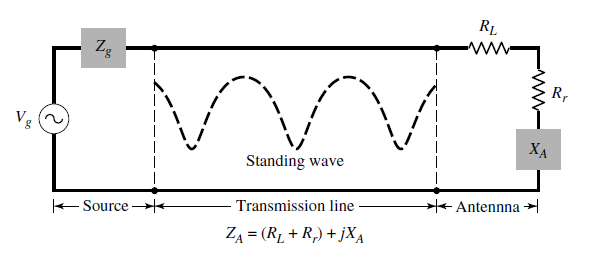
\includegraphics[scale=0.8]{circuit_model_antenna}
		\caption{Spherical coordinate system components}
		\label{fig:circuit_model_antenna}
	\end{figure}
    
    The Fig.\ref{fig:circuit_model_antenna} shows transmitter mode antenna model. The receiver mode model of the antenna is similar to this one, but the source is changed with the receiver. +
     
    In order to provide radiation, a disturbance is required. That disturbance is the time-varying current. In addition to the disturbance, the continuity of the electric field completes the radiation process. In guiding device, the particle travels back and forth.   
    
    \begin{figure}[h]
		\centering
		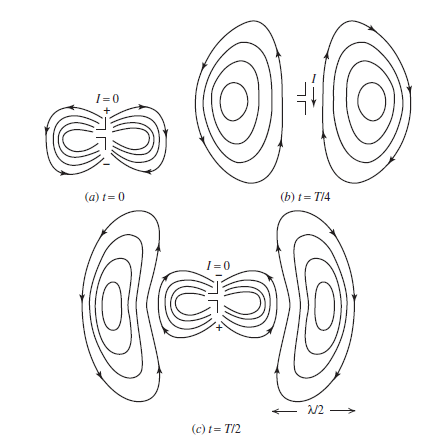
\includegraphics[scale=0.6]{dipol}
		\caption{Oscillating dipol and creation of the electric field lines for different time instants}
		\label{fig:dipol}
	\end{figure}
    
    \newpage
    
    \section{Antenna Types}
    \paragraph~ In this section the four fundamental antenna type is analyzed. Antenna name which belongs to one of the four type will be classified.
    
    \subsection{Electrically Small Antennas}
    \paragraph~ Physical length of the these antennas are greater than one fiftieth of the wavelength. Input impedance of these antennas have low resistance and high reactance. Vertical monopole used in AM reception on cars is an example. Short dipole and small loop are other examples. 
    \subsection{Resonant Antennas}
    \paragraph~ They have simple structure, good input impedance, narrow bandwidth. In these antennas main beam is broad. Half-wave dipole is well-known example.   
    \subsection{Broadband Antenna}
    As its name implies, they operates over wide frequency range.  The term active region is an important parameter in the characterization of these antennas.  
    \subsection{Apperture Antenna}
    \section{Antenna Parameters}

    \subsubsection{Radiation Pattern}

    \paragraph~ Antenna radiation pattern provides the information that how the antenna radiates the waveform at its feedline through the ambiance. To obtain radiation pattern of an antenna, analysis of \textbf{E} and \textbf{H} fields are required. Equation(1.1) represents the \textbf{E} field, radiated by an antenna, in the far-field region.  Therefore, pattern functions $F_{ \phi}( \theta, \phi)$ and $F_{ \theta}(\theta,\phi)$ do not depend on the distance $R$ from the antenna.
		
    \begin{equation}
		E(R,\theta,\phi)=[\hat{\theta}F_{ \phi}( \theta, \phi)+ \hat{ \phi}F_{ \theta}(\theta,\phi)]\frac{e^{-jk_oR}}{R}
	\end{equation}
	
	where $k_o=\frac{2\pi}{\lambda}$ is free space propagation constant. 
	\begin{figure}[h]
		\centering
		\includegraphics[scale=0.8]{spherical_coor }
		\caption{Spherical coordinate system components}
		\label{fig:spherical}
	\end{figure}
	
	The pattern function is related with the voltage. As a result, it constitutes the radial scale of the radiation pattern with the Eq.(\ref{eq:pattern_func}).
	
	\begin{equation}
		20log(|F(\theta,\phi)|)
		\label{eq:pattern_func}
	\end{equation}
	
	\paragraph~ Detection of a pattern function requires rotating the  antenna either in the  transmitter or in the receiver operation. This is due to parameters of the pattern function. By rotating the antenna, \textbf{E} and \textbf{H} fields are observed at \textit{$\theta$} and \textit{$\phi$} by keeping the \textit{R} constant.
	
	\paragraph~ Magnitude scale of the radiation pattern can be chosen as either field pattern and power pattern. The field pattern is drawn in linear scale. Also, the power pattern can be drawn either in linear scale or desibel scale. 
	
	\newpage
	
	\paragraph~ Drawing the pattern in any of the scaling factor only changes the coefficients which correspond to the half power beamwidth (HPBW) point. If a field pattern is drawn in linear scale, HPBW points correponds to 0.707 value. If a power pattern is drawn in linear scale, this point (HPBW) represents 0.5, where the power is halved. This is another way of representing -3dB point in dB scale.
	
	
	
	\begin{figure}[h]
		\centering
		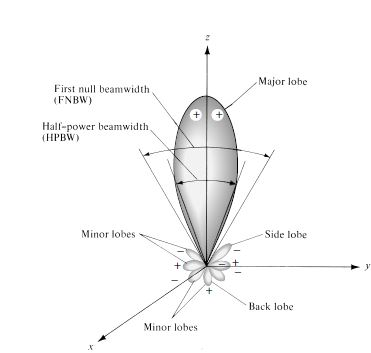
\includegraphics[scale=1.2]{rad_patt}
		\caption{Radiation pattern of a directional antenna \cite{1}}
		\label{fig:rad_patt}
	\end{figure}
	
	\paragraph~ In the Fig.\ref{fig:rad_patt}, pattern function is visualized in polar plot. Also, it is possible to draw the diagram in rectangular form to make the minor lobes more observable. The major lobe represents the direction of maximum radiation. The remaining lobes are called as minor lobes. Side lobe is the one which shows up adjacent to the main lobe. Finally, there is 180$\degree$ between main lobe and back lobe.
	
	\paragraph~ The Fig.\ref{fig:rad_patt} shows directional antenna behavior, which has a relatively large major lobe. In addition, there are isotropic and omnidirectional pattern types. Isotropic pattern shows an ideal, lossless antenna which radiates equally in all directions, which is not realizable. Also, the omnidirectional pattern is radiation characteristic belong to an antenna which has a nondiretional pattern in a given plane and directional pattern to the orthogonal plane. 
	
	\newpage
	
	\paragraph~ The field characteristic changes around the space of an antenna. There are mainly three field regions: reactive near-field, radiating near-field (Fresnel), far-field (Fraunhofer). The regions and their mathematically determined boundaries can be seen in Fig.\ref{fig:field_regions}.
	
	\begin{figure}[h]
		\centering
		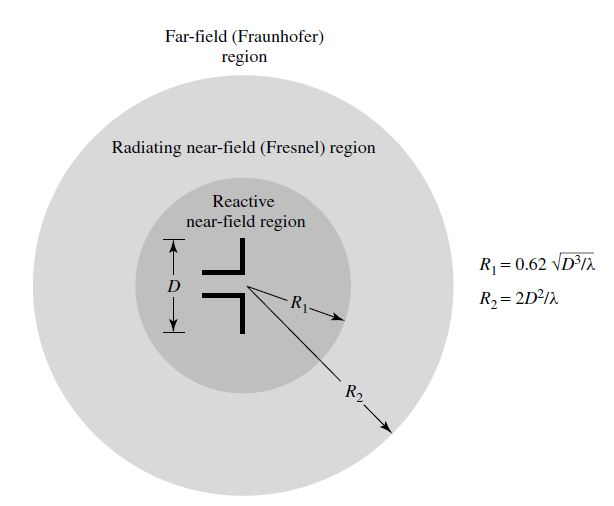
\includegraphics[scale=0.8]{field_regions}
		\caption{Antenna amplitude pattern change for different field regions  \cite{1}}
		\label{fig:field_regions}
	\end{figure}
	
	\subsection{Radiation Power Density}
	
	The radiated power in an antenna gives an insight about the wireless link. The instantaneous power in an electromagnetic wave is,
	
	\begin{equation}
	    W=E \times H
	\end{equation}
	
	Here, \textit{W} instantaneous poynting vector in W/m$^2$, \textit{E} instantaneous electric-field intensity in V/m, \textit{H} instantaneous magnetic-field intensity in A/m. 
	
	By applying surface integration to the power density, it is possible to obtain instantaneous total power,
	
	\begin{align*}
       P = \oiint\limits_S \VF{W} \cdot \dif s
       &= \oiint\limits_{S} \VF{W} \cdot \hat{\VF{n}} \dif a\\
    \end{align*}
	
	Here, \textit{P} is instantaneous total power in watts (\textit{W}), $\hat{\VF{n}}$ is  unit vector normal to the surface and \textit{da} is infinitesimal area of the closed surface in \textit{m$^2$}. This integral contains complex parts, so using the phasor notation, the average power radiated by an antenna can be calculated as
	
	\begin{equation}
	    P_{rad} = \frac{1}{2} \oiint\limits_S Re(E \times H^*) \cdot \dif{\VF{s}}
	\end{equation}
	
	\subsection{Radiation Intensity}
	
	\paragraph~ Radiation intensity is the interpretation of the radiated power by considering unit solid angle. It is far-field parameter and  represented mathematically as,
	
	\begin{equation}
	    U = r^2 W_{rad}
	\end{equation}
	
	where \textit{r} is the distance from an antenna and \textit{W$_{rad}$} is the radiation density.
	
	\newpage
	
	\subsection{Beamwidth}
	
	\paragraph~ Beamwidth of an antenna is obtained from the radiation pattern. It is the angular distance between two symmetrical points, where the symmetry axis is chosen as the peak point of the main lobe. HPBW is emphasized before as the points where the power the of the main peak is halved. In addition, first-null beamwidth is the angular seperation of the first nulls of the pattern.
	
	However, the term \textit{beamwidth} refers to as HPBW.
	
	\subsection{Directivity}
	
	Previously, the radiation intensity of an antenna was explained. Here, directivity is an some type of the interpretation of radiation intesity. Directivity provides the comparision between the radiation intensity in a given direction with radiation intensity over all directions. This ratio gives the directivity.
	
	\begin{equation}
	    D = \frac{U}{U_o} = \frac{4\pi U}{P_{rad}}
	\end{equation}
	
	where D is directivity (dimensionless), U is radiation intensity (W/unit solid angle),  U$_o$ is radiation intensity of isotropic source (W/unit solid angle), P$_{rad}$ is total radiated power (W).
	
	\paragraph~ Directivity of an antenna may be calculated experimentally by using numerically derived Kraus equation in Eq.\ref{eq:kraus}, 
	
	 \begin{equation}
        	D_0=\frac{41,253}{\theta_{1r}\theta_{2r}}
        	\label{eq:kraus}
    \end{equation}
    
    or Tai-Pereira equation in Eq.(\ref{eq:tai-pereira}),
    
    \begin{equation}
    		D_0=\frac{22,181}{\theta_{1r}^2+\theta_{2r}^2}
    		\label{eq:tai-pereira}
    	\end{equation}
	
	where $\theta_{1r}$ and $\theta_{2r}$ stands for the -3dB power points of the received power in radians.
	
	\subsection{Antenna Efficiency}
	
	\paragraph~ There are several losses in an antenna and they forces to define antenna efficiency. The losses can be grouped as I$^2$R losses, which turns into heat, and reflection losses due to the mismatch between antenna and the feeding network. Antenna efficiency is dimensionless and defined as,
	
	\begin{equation}
	    e_o = e_r e_c e_d
	    \label{eq:antenna_eff}
	\end{equation}
	
	where e$_o$ is total efficiency, e$_r$ is reflection (mismatch) efficiency ($1-|\Gamma|^2$), e$_c$ is conduction efficiency, e$_d$ dielectric efficiency. 
	
	Calculation of the e$_c$ and e$_d$ is cumbersome. They can be measured experimentally. Also multiplication of them is used to relate gain and directivity parameters.
	
	\subsection{Gain}
	
	\paragraph~ One of the important property of an antenna is its gain. The calculation of the gain carries considerable information about the wireless link. The point, which gain and directivity differs, is that gain additionally covers the antenna efficiency together with the directional capabilities of an antenna. 
	
	There are several methods for the experimentally calculation of an antenna gain, absolute gain method uses the Eq.\ref{eq:friis} which is  
	
	\begin{equation}\label{eq:friis}
			P_r=P_oG_{0t}G_{0r} \bigg(\frac{\lambda}{4\pi R}\bigg)^2
	\end{equation} 
	
	where $P_r$ is received power, $P_o$ is the power fed to the transmitting antenna, $G_{0t}$ and $G_{0r}$ are the gains of the transmitting and the receiving antennas, respectively. $R$ is the distance from the antenna under concerned and $\lambda$ is the wavelength at the operating frequency. $(\frac{\lambda}{4\pi R})^2$ is the part which represents free-space radiative loss.
	
	\newpage
	
	\subsection{Beam Efficiency}
	
	\paragraph~ In the beam efficiency, major lobe power is compared with the total power radiated by the antenna. It is dimensionless.
	\begin{equation}
	    BE=\frac{Power \: transmitted \: (received) \: within \: cone \: angle \: \theta_1}{Power \: transmitted \: (received) \:  by \: the \: antenna}
	\end{equation}
	
	\subsection{Bandwidth}
	\paragraph~ It is considered as the frequency range between upper and lower cut-off frequencies around the center frequency. The center frequency of an antenna is considered as the resonance frequency. In this range antenna characteristics are as expected in early design stages. 
	
	Broadband antenna bandwidth is expressed as the upper-to-lower frequency ratio. For instance 10:1 indicates that upper frequency is 10 times greater than lower frequency. However, approach is different for narrowband antennas. They are expressed as  the frequency difference of upper and lower frequencies over the center frequency. For example, 10\% means that bandwidth is the 10\% of the frequency difference around the center frequency. 
	
	\subsection{Polarization}
	
	\paragraph~ Polarization of an antenna is considered as the polarization of an electromagnetic wave radiated by the antenna under concern. Polarity of an electromagnetic wave is related with the time-varying direction of the electric field vector and its relative magnitude. Polarization of antenna is so important that, in a wireless link, if the polarization mismatch occurs between transmitted and the received antennas data transmission can not be provided. Polarization in electromagnetic wave can be classified as linear, circular and elliptical polarizations.
	
	\subsection{Input Impedance}
	
	\paragraph~ As its name implies, input impedance of an antenna is the ratio of an voltage and current at its terminals or the ratio of the electric and magnetic fields at its corresponding terminals (depending on the transmitter-receiver operations). 
	
    \begin{equation}
        Z_A = R_A+jX_A = R_r + R_L + jX_A
    \end{equation}
	
	where $R_A$ and $X_A$ are the real and imaginary parts of the antenna impedance $Z_A$, as seen through its terminals. $R_r$ is the radiation resistance of the antenna. $R_L$ is loss resistance of the antenna.
	
	\paragraph~ The antenna efficiency can be increased by the reduction of the reflective losses. This can be achieved by simply conjugate matching between feeding network and antenna. In this way, loss can be minimized.
	
	\subsection{Antenna Radiation Efficiency}
	
	As it was mentioned earlier, the calculating of antenna radiation efficiency is cumbersome. Instead, it is measured experimentally. It is determined by the radiation resistance and the loss resistance, from the thevenin or norton equivalent of an antenna.
	
	\begin{equation}
	    e_{cd}= \frac{R_r}{R_r+R_L}
	\end{equation}
	
	\newpage
    \renewcommand\bibname{References}
    \addcontentsline{toc}{chapter}{REFERENCES}
    \begin{thebibliography}{5}
	    \bibitem{1} BALANIS, C. A., \underline{Antenna Theory: Analysis and Design}, Wiley-Interscience, 3th edition, 2005.
	\end{thebibliography}
\end{document}
